% Gemini theme
% https://github.com/anishathalye/gemini

\documentclass[final]{beamer}

% ====================
% Packages
% ====================

\usepackage[T1]{fontenc}
\usepackage{lmodern}
\usepackage[size=custom,width=109,height=107,scale=1.0]{beamerposter}
\usetheme{gemini}
\usecolortheme{gemini}
\usepackage{company-poster}
\usepackage{graphicx}
\usepackage{booktabs}
\usepackage{tikz}
\usepackage{pgfplots}
\pgfplotsset{compat=1.14}
\usepackage{anyfontsize}

% ====================
% Lengths
% ====================

% If you have N columns, choose \sepwidth and \colwidth such that
% (N+1)*\sepwidth + N*\colwidth = \paperwidth
\newlength{\sepwidth}
\newlength{\colwidth}
\setlength{\sepwidth}{0.025\paperwidth}
\setlength{\colwidth}{0.3\paperwidth}

\newcommand{\separatorcolumn}{\begin{column}{\sepwidth}\end{column}}

% ====================
% Title
% ====================

\title{Streamlining Automated Laboratory Workflows in Tightly Firewalled Networks }

\author{Eli J. Fine \inst{1} \and Stephen Dambman \inst{1} \and Nathan Zender \inst{1} \and Calvin Sy \inst{1} \and Steve Testen \inst{1} \and David Dambman \inst{1}}

\institute[shortinst]{\inst{1} Lab Sync Inc., San Diego, CA} % TODO: consider removing institute if we want some more space

% ====================
% Footer (optional)
% ====================

\footercontent{
  \href{https://www.lab-sync.com}{https://www.lab-sync.com} \hfill
  Society for Laboratory Automation \& Screening 2026, Boston, MA, USA --- 1052-C \hfill
  \href{mailto:eli.fine@lab-sync.com}{eli.fine@lab-sync.com}}
% (can be left out to remove footer)

% ====================
% Logo (optional)
% ====================

% use this to include logos on the left and/or right side of the header:
% \logoright{\includegraphics[height=7cm]{logo1.pdf}}
\logoleft{
\includegraphics[height=6cm]{lab-sync-primary-bw.pdf}}

% Overview: A succinct summary of the purpose, methods, and results. Use phrases rather than sentences in a simple outline format.
%Introduction: A concise statement of the objective and background of the work.
%Methods: Describe the apparatus, chemistry, samples, and materials used in detail.
%Results: Use graphs, spectra, charts, and pictures with a minimum of text to illustrate results.
%Conclusions: Concise statement of the findings indicating future research directions.

% ====================
% Body
% ====================

\begin{document}

\begin{frame}[t]
\begin{columns}[t]
\separatorcolumn

\begin{column}{\colwidth}

  \begin{block}{Overview}
Purpose
    \begin{itemize}
      \item \textbf{Compliance} with security posture required by Information Technology and Operational Technology teams
      \item \textbf{Observability} of instrument alerts even when firewall blocks traditional alerting mechanisms
      \item \textbf{Traceability} of changes to methods and configuration using version control even when firewall blocks access to company Git servers 
      \item \textbf{Straightforward} installation requiring little technical knowledge
      \item \textbf{Seamless} use by scientists and engineers with limited experience using version control
    \end{itemize}

    Methods
    \begin{itemize}
      \item \textbf{Containerized and open-source} applications to facilitate security scanning and limit required privileges
      \item \textbf{k3s container management} to enable license-free robust deployment to Windows or Linux systems
      \item \textbf{SMTP sink server} to capture emails within the firewall
      \item \textbf{Self-hosted Git server} within firewall
      \item \textbf{Purpose-built `Git Sherpa'} application to guide user interaction with Git and transfers across the air-gap
    \end{itemize}

    Results
    \begin{itemize}
      % \item \textbf{Version control} within the lab allowed tracking changes and rapid transitions between test and production code.
\item \textbf{Reduced downtime} for scheduler upgrades via branch-based rollout and rapid rollback.
  \item \textbf{Faster propagation} of method and configuration changes across workcells, replacing manual file drops.      
      \item \textbf{Improved auditability} with an end-to-end trace of what changed, when, and by whom across the lab.
      \item \textbf{Simulation environments} were able to be set up outside the firewall and synchronized with the lab environment using Git Bundles
      \item \textbf{Aggregated alerting} from many sources allows easy viewing and a single point to manage forwarding to any allowed external services.      
    \end{itemize}

  \end{block}

  \begin{block}{Introduction}

    High-throughput laboratories operating within air-gapped or tightly firewalled networks face significant operational hurdles. Manual file transfers for method updates, divergence between development and production environments, and limited visibility into code and configuration changes lead to errors and impede development. Furthermore, critical instrument alerts are often trapped behind the firewall, preventing timely operator notification. We describe approaches using freely available open-source tooling developed by ourselves and others that address these problems. The framework minimizes manual steps and human error while preserving the strict security posture of network isolation. 

    Prior to implementing this solution, a large orchestrated laboratory---with numerous workcells interconnected by tracks and mobile robot transport systems---was encountering several major pain points.  Small changes made in one workcell caused issues elsewhere because the impacts were not visible to other engineers on the team more familiar with different parts of the lab.  Developing new workflows required taking the lab out of commission---even to run basic simulation tests---because managing a digital twin was prohibitively difficult. Upgrading the scheduling software was deferred because the time required to upgrade all the workcells and test all the workflows was prohibitively long, as it would disrupt active processing of samples. Alerts from device and scheduling software were all funneled to the single email address allowed through the firewall, resulting in an unhelpful firehose of information that was overwhelming to triage. 
    
    Many of these issues are addressable by using version control.  However, the firewall prevented access to SaaS solutions (e.g. GitHub, Bitbucket). 

    A further challenge common in many laboratories is a lack of access to Linux servers commonly used to run modern software applications. In many cases, the only available option is a standard Windows 11 (or in many cases Windows 10) PC.

    Any solution to streamline automated laboratory workflows under increasingly stringent security constraints must therefore be able to operate on Windows, without access to external internet, not require administrative privileges on any computer, and ideally be open and scannable by security teams to probe for any weaknesses that threat actors could exploit to compromise the discoveries being made or therapeutics being manufactured.

  \end{block}

\end{column}

\separatorcolumn

\begin{column}{\colwidth}

  \begin{block}{Methods}

    \heading{Installation}
    The central applications (Nexus Notifications Center, Mailpit, Gitea) all run as containerized services in a lightweight k3s environment (e.g. Rancher Desktop) compatible with Windows 10/11 or Linux. `Git Sherpa' can be installed as a background service running on Windows 10/11 or Linux. All applications provide browser-based user interfaces that are accessible from any computer within the tightly firewalled environment.
    \heading{Architecture}
    

    \begin{figure}
      \centering
      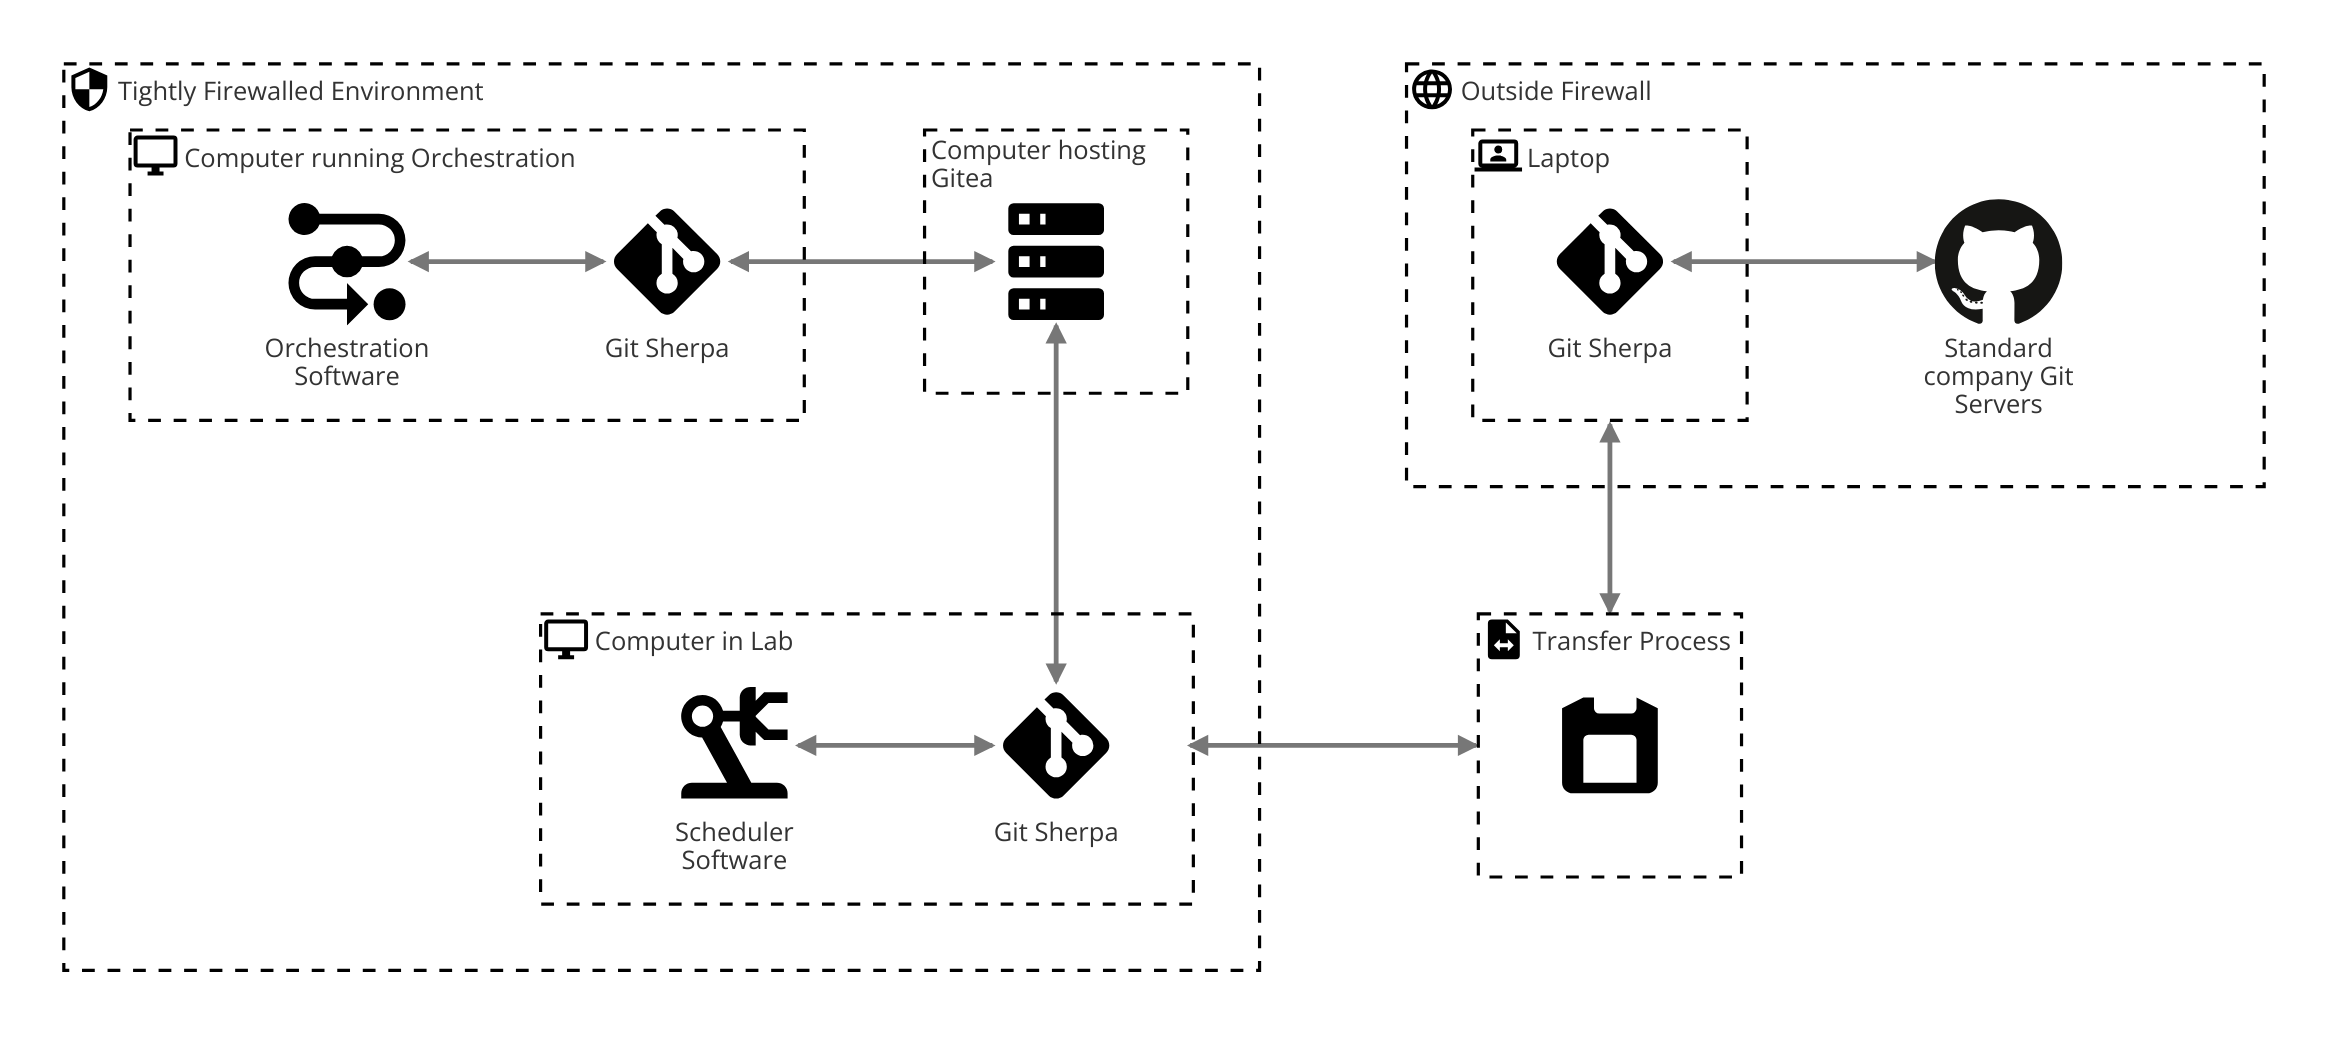
\includegraphics[width=33cm]{figures/git-architecture.png}
      
      \caption{\textbf{Version control architecture.} An instance of `Git Sherpa' runs on each computer in the lab to facilitate version control of the programs and configuration. `Git Sherpa' synchronizes with the instance of Gitea. If desired, any instance of `Git Sherpa' can export/import bundles to transfer across the air-gap, where another instance of `Git Sherpa' can interface with the standard company Git server.}
    \end{figure}

    \begin{figure}
      \centering
      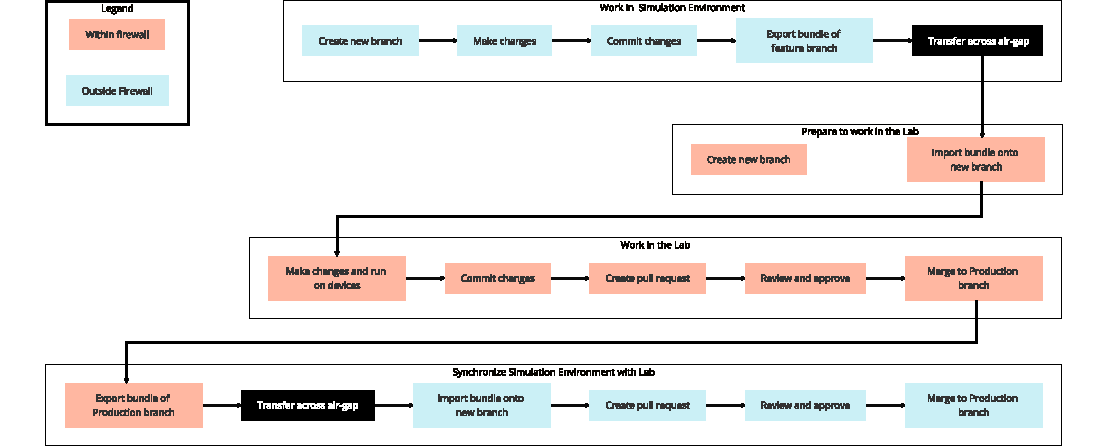
\includegraphics[width=33cm]{figures/git-flow.pdf}
      
      \caption{\textbf{Git Flow}. `Git Sherpa' can be utilized to transfer work to and from a simulation environment outside the air-gap. If no simulation environment is desired, then a standard Git flow can be utilized purely within the lab by creating a new branch in the lab to begin new work after merging to production.}
    \end{figure}

    \begin{figure}
      \centering
      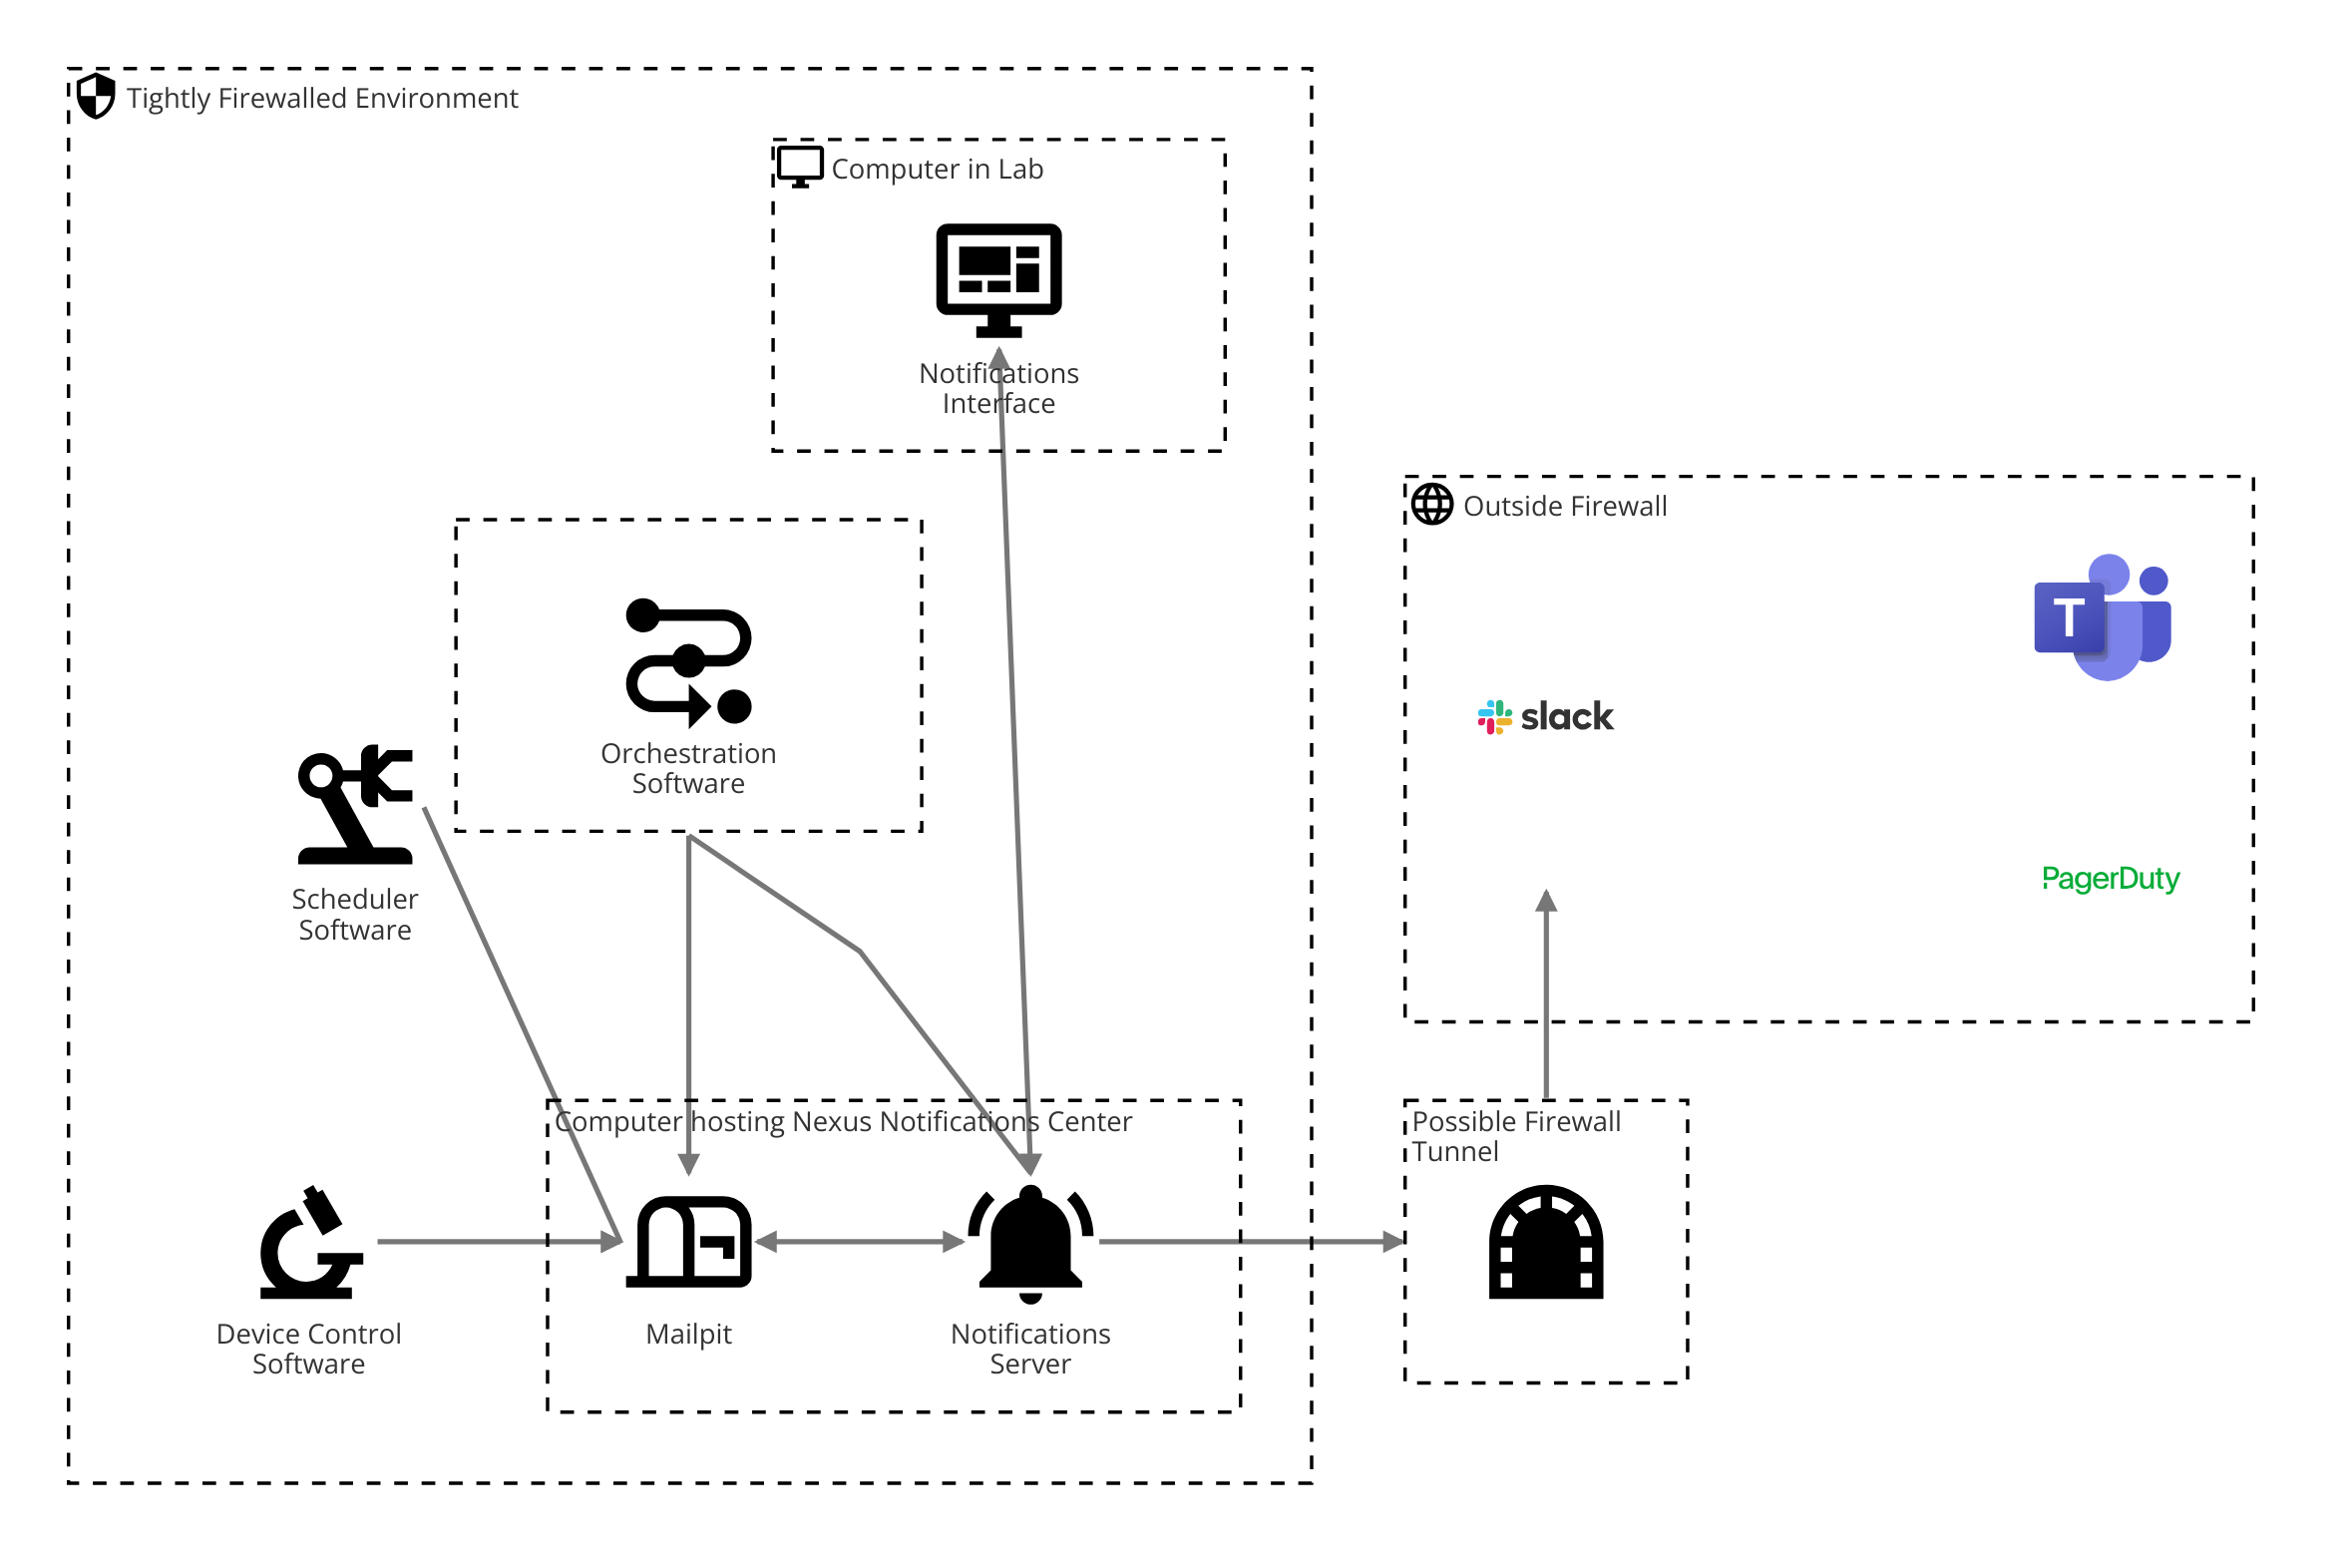
\includegraphics[width=33cm]{figures/nexus-architecture.png}
      
      \caption{\textbf{Observability Architecture.} An instance of Mailpit and the Nexus Notifications Center are deployed. Vendor software that can only send alerts via email can be pointed at the Mailpit receiving address. Software can also create alerts by directly calling the Nexus API. On any computer in the lab, users can view the Notifications Center dashboard. If available, the Notifications server can relay aggregated alerts through a tunnel in the firewall to an external service.}
    \end{figure}

  \end{block}

\end{column}

\separatorcolumn

\begin{column}{\colwidth}

  \begin{block}{Results}

    \begin{figure}
      \centering
      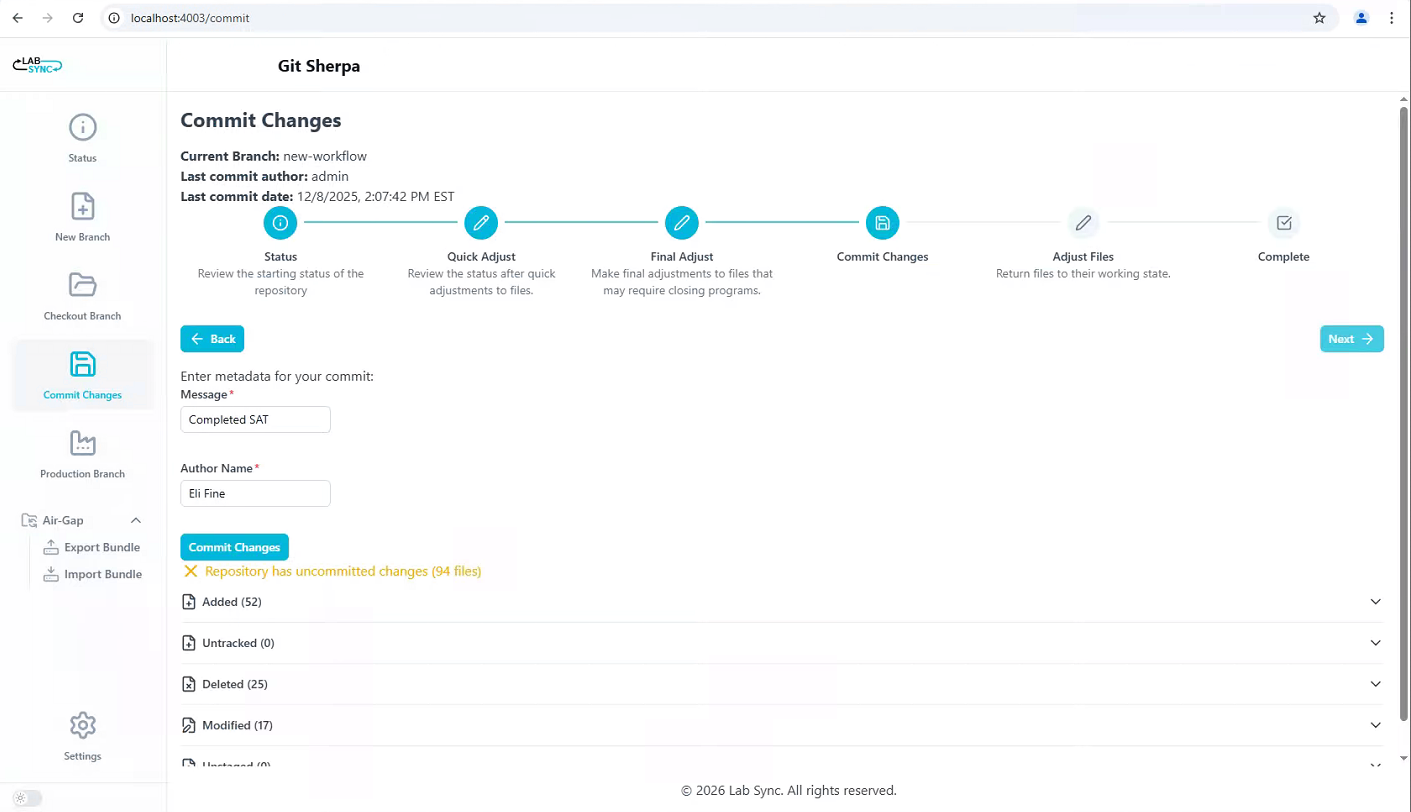
\includegraphics[width=33cm]{figures/commit-light.png}
      
      \caption{The `Git Sherpa' application runs as a background service on the computers with automation software in order to track those files. It is accessible as a web application from anywhere in the lab. It guides users through step-by-step workflows for utilizing version control and transferring bundles across the air-gap.}
    \end{figure}

    \begin{figure}
      \centering
      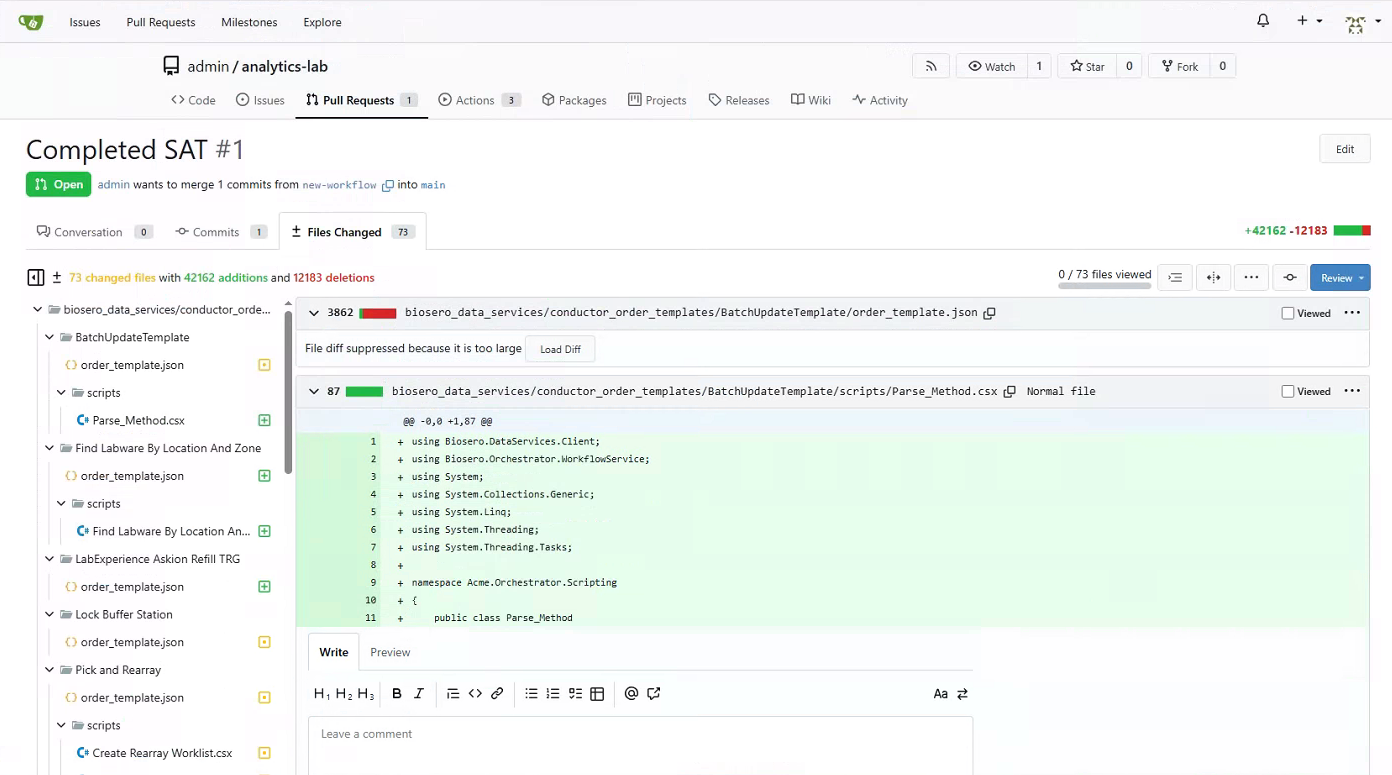
\includegraphics[width=33cm]{figures/pr-light.png}
      
      \caption{Gitea operates as the remote Git server inside the firewall. It has a fully featured user interface to allow operations including pull requests, approval rules, and authentication.}
    \end{figure}

    \begin{figure}
      \centering
      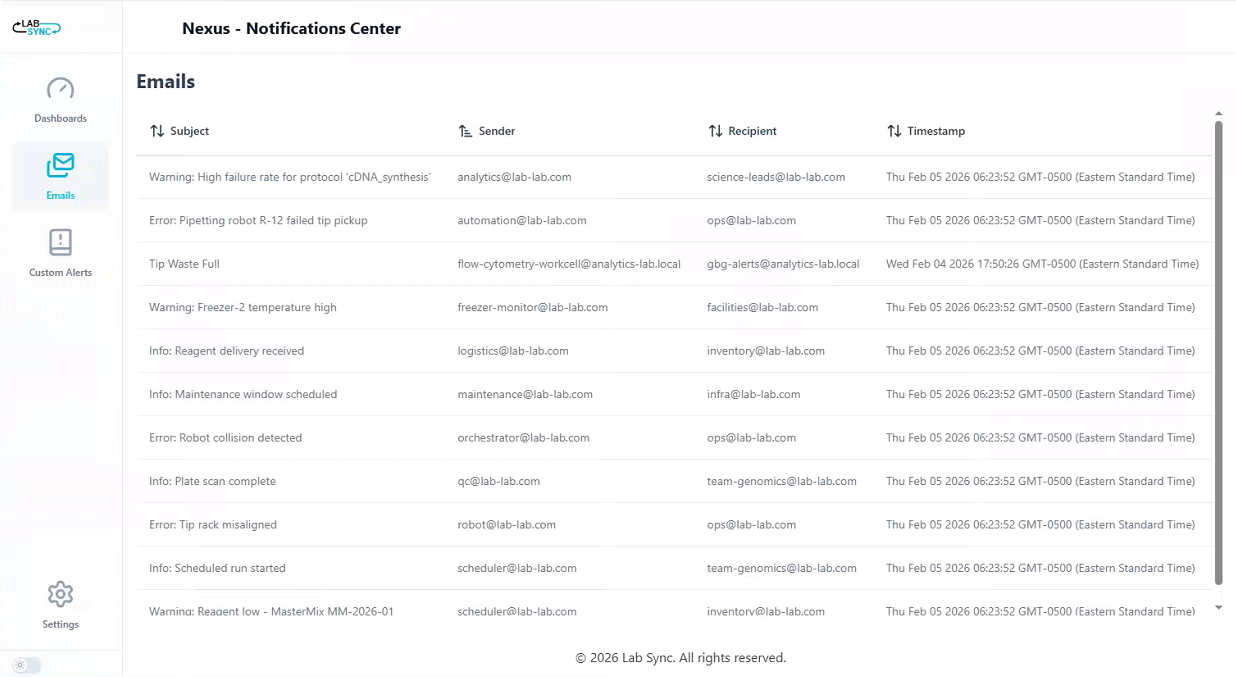
\includegraphics[width=33cm]{figures/notifications-light.png}
      
      \caption{The Nexus Notifications Center summarizes alerts sent via email or the API endpoint in a user interface accessible anywhere in the lab. It can also serve as a conduit for custom logic to forward notifications through a specific tunnel allowed through the firewall.}
    \end{figure}

  \end{block}

  \begin{block}{Conclusions}

    Increasingly stringent security postures are a growing challenge for laboratory automation as IT policies formerly reserved for manufacturing facilities make their way into R\&D laboratories, and as laboratory automation begins to make inroads into the manufacturing environment.

    We demonstrated approaches to handle two critical aspects of a high-throughput lab that have historically been managed by direct connection to services running in the cloud: observability of incidents and version control of methods.

    By building open-source tooling, we hope to allow easy security scrutiny of the approaches and enable community contributions to accelerate progress.

  \end{block}

\end{column}

\separatorcolumn
\end{columns}
\end{frame}

\end{document}
